\documentclass[a4paper,10pt]{article}
\usepackage[utf8]{inputenc}
\usepackage[default]{raleway}
\usepackage{geometry}
\usepackage{enumitem}
\usepackage{multicol}
\usepackage{titlesec}
\usepackage{graphicx}

% Marges du document
\geometry{margin=1in}

% Format des sections
\titleformat{\section}{\large\bfseries}{}{0em}{}[\titlerule]
\titleformat{\subsection}{\bfseries}{}{0em}{}

\begin{document}

% Tête du CV
\begin{center}
    \Huge{\textbf{Narimane Zaouache}} \\
    \large{Étudiant en M1 Calcul Scientifique et Mathématiques de l'Information} \\
    \vspace{0.2em}
    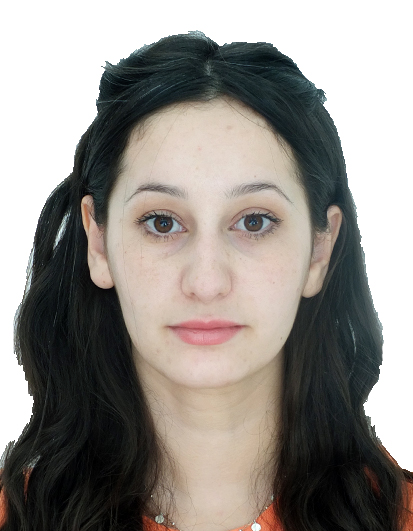
\includegraphics[width=4cm, height=4cm]{profile_image.jpg} % Assurez-vous que le fichier image est téléchargé
\end{center}

% Coordonnées
\section*{Coordonnées}
\begin{tabular}{rl}
    \textbf{Adresse :} & 22 Rue de Bouxwiller, 67000, Strasbourg \\
    \textbf{Téléphone :} & 0753339394 \\
    \textbf{Email :} & narimanezaouache703@gmail.com \\
    \textbf{Permis :} & Permis B \\
\end{tabular}

% Profil
\section*{Profil}
Étudiant en Master de Calcul Scientifique et Mathématiques de l'Information. Je suis créative, autonome et coopérative. Passionnée par les défis mathématiques et d'informatique, je suis capable de travailler de manière autonome en équipe pour contribuer à des projets novateurs.

% Expérience
\section*{Expérience}
\subsection*{Gestionnaire, 01/2022 - 08/2023}
\textbf{SNC BEN HAMLAT} transport des produits pétroliers et de gaz - Tizi Ouzou - CDI
\begin{itemize}[leftmargin=*]
    \item Rédaction précises des factures.
    \item Gestion des stocks.
    \item La programmation et le suivi d'entretien des engins.
    \item Suivi méticuleux du personnel.
    \item Traitement rapide et précis des plaintes d'assurance pour le personnel.
    \item Préparation rigoureuse des dossiers.
\end{itemize}

\subsection*{Serveuse}
\begin{itemize}[leftmargin=*]
    \item Assurer que les besoins des clients soient pleinement satisfaits en fournissant un service rapide et courtois lors des événements.
    \item Travailler en équipe avec les collègues pour assurer une expérience client optimale.
\end{itemize}

% Formation
\section*{Formation}
\begin{itemize}[leftmargin=*]
    \item \textbf{Master 1 :} Calcul scientifique et mathématiques de l'information, 2024/2025, Université de Strasbourg - Strasbourg.
    \item \textbf{Master 2 :} Recherche Opérationnelle, 09/2020 - 07/2022, Université Mouloud Mammeri - Tizi Ouzou.
    \item \textbf{Licence :} Mathématiques, 09/2016 - 07/2020, Université Mouloud Mammeri - Tizi Ouzou.
    \item \textbf{Baccalauréat :} Science Expérimentale, 09/2014 - 07/2015, Direction de l'éducation-Draâ El Mizan - Tizi Ouzou - ASSEZ BIEN.
\end{itemize}

% Compétences
\section*{Compétences}
\begin{itemize}[leftmargin=*]
    \item Analyse et gestion des données : Excel, SQL, Python (y compris NumPy, Pandas, gestion de base de données), C++, C, Julia.
    \item Outils de versement et collaboration : Git, GitHub.
    \item Création de rapports et présentations : LaTeX, Word, PowerPoint.
    \item Résolution des problèmes.
    \item Analyse des données.
\end{itemize}

% Centres d'intérêt
\section*{Centres d'intérêt}
\begin{itemize}[leftmargin=*]
    \item Cinéma
    \item Lecture
    \item Sport
    \item Réseaux sociaux
\end{itemize}

% Langues
\section*{Langues}
\begin{itemize}[leftmargin=*]
    \item Arabe : Expérimenté (C2)
    \item Français : Courant (C2)
    \item Anglais : Intermédiaire
    \item Kabyle : Langue maternelle
\end{itemize}

% Certifications
\section*{Certifications}
\begin{itemize}[leftmargin=*]
    \item Attestation en Maintenance Informatique et Installation Réseaux - 2019
    \item Attestation The 21st Century Skills Training - 2022
\end{itemize}

\end{document}
